\documentclass[11pt]{article}
\usepackage{graphicx}
\usepackage{geometry}	
\usepackage{amssymb}
\usepackage{float}
\usepackage{caption}
\usepackage{subcaption}
\usepackage{amsmath}
\usepackage{amssymb}


\begin{document}


\begin{center}
{\bf{\huge{Motion Control Manual for pSCT Telescope}}}

\vspace{0.1in}
Last updated July, 2016

\vspace{0.3in}
{\it{\underline{Abstract:}}} We detail the operation and troubleshooting methods for the telescope motion control system.

\end{center}

\tableofcontents

\vspace{0.2in}


\section{Overview}

This manual details the system in place to move and align the prototype SCT telescope camera.
Figure \ref{FigWhole} shows a system overview schematic.
The camera can be roughly broken up into two main structural components, the outer structure and the inner structure.
The camera outer structure does not move and rigidly connects to the rest of the telescope (via the octagon - shown in yellow in Fig. \ref{FigWhole}).
The inner structure consists of the camera itself, the associated electronics, and the thermal management system.
The inner structure is movable and is connected to the outer structure by three ball pin joints, one on the top and two on the bottom.
The inner structure is supported and positioned only via these three ball pins.


\begin{figure}[h]
\begin{center}
\includegraphics[width = 4.5in]{camerapicNew.png}
\caption{Motor labels and setup as defined from looking at the camera from the front.}  
\label{FigWhole}
\end{center}
\end{figure}

Figure \ref{FigMotor} shows in detail one of the three motor assemblies.
Motion is controlled in each assembly by a stepper motor that twists a motor driver screw.
The twist of this screw pushes or pulls a flange rigidly connected to the ball pin assembly.
The motion of this ball pin assembly is restricted to an axis defined by a rail system.
The driver screw and rails must be parallel for this to work well.
One step from a stepper motor corresponds to $\sim$1.02 micron of motion along this axis for the ball pin.
The total range of motion is 5 cm along this direction (z).

Conversely, motion along the x/y axis is performed manually.
With the horizontal alignment screws loose, the ball pin can move along a track perpendicular to the rails (see Fig. \ref{FigMotor}).
However, there is no stepper to help with horizontal shifts.
Additionally, the vertical alignment screws above and below the ball pins control the up/down positioning.
The total allowed motion along these axes is 2.5 cm.

A web interface is hosted on an Arduino Yun to command the three steppers.
The Yun is housed in an electronics control box (see Fig. \ref{FigElecBox}) that is mounted near the bottom of the back plane of the camera lattice.
The wiring diagram for this electronics control box is shown in Fig. \ref{elecFit}.

\begin{figure}[h]
\begin{center}
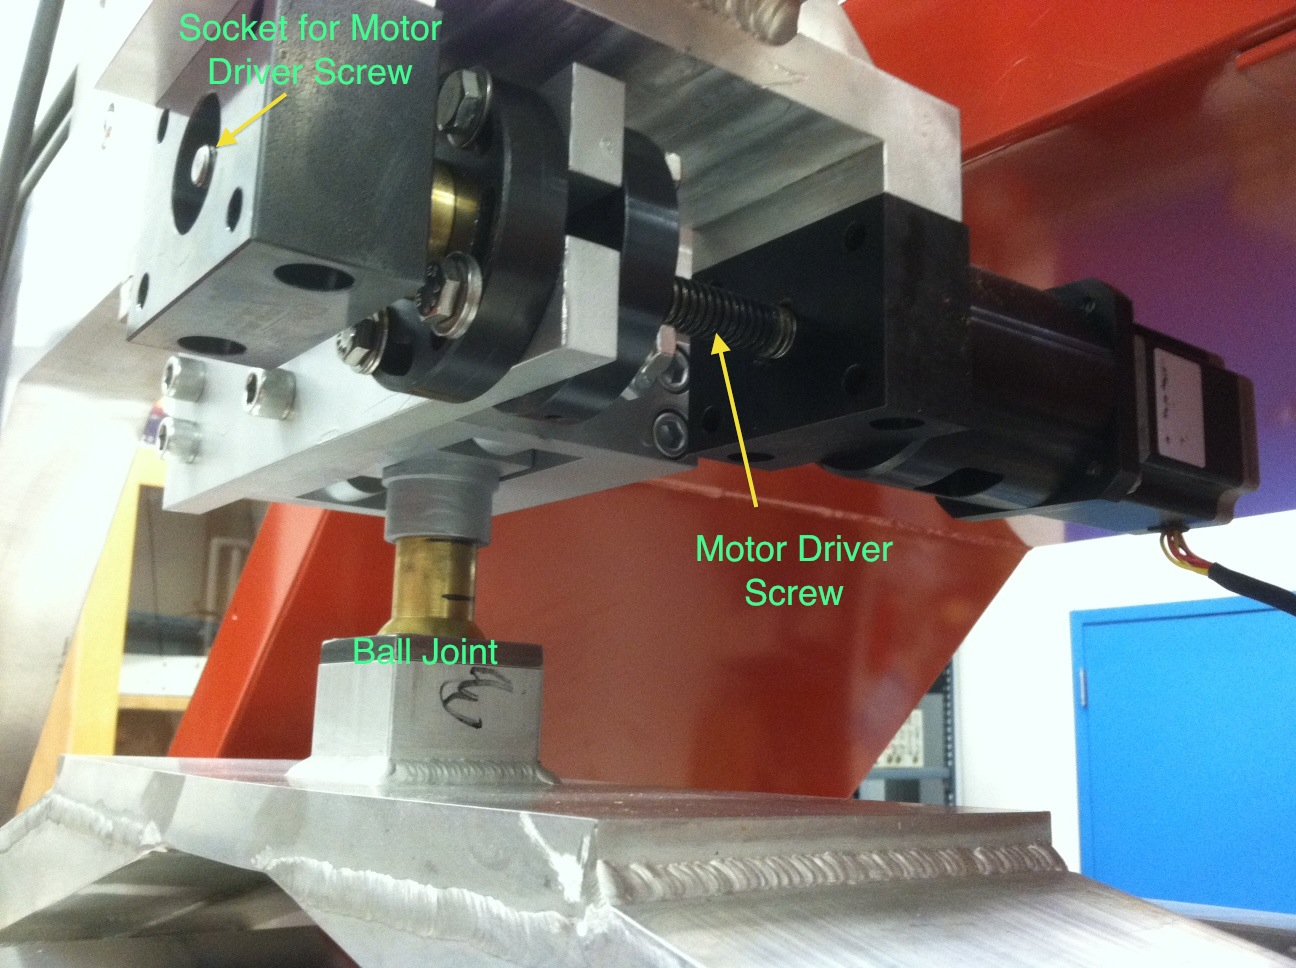
\includegraphics[width = 2.6in]{motorAss1Edit.JPG}
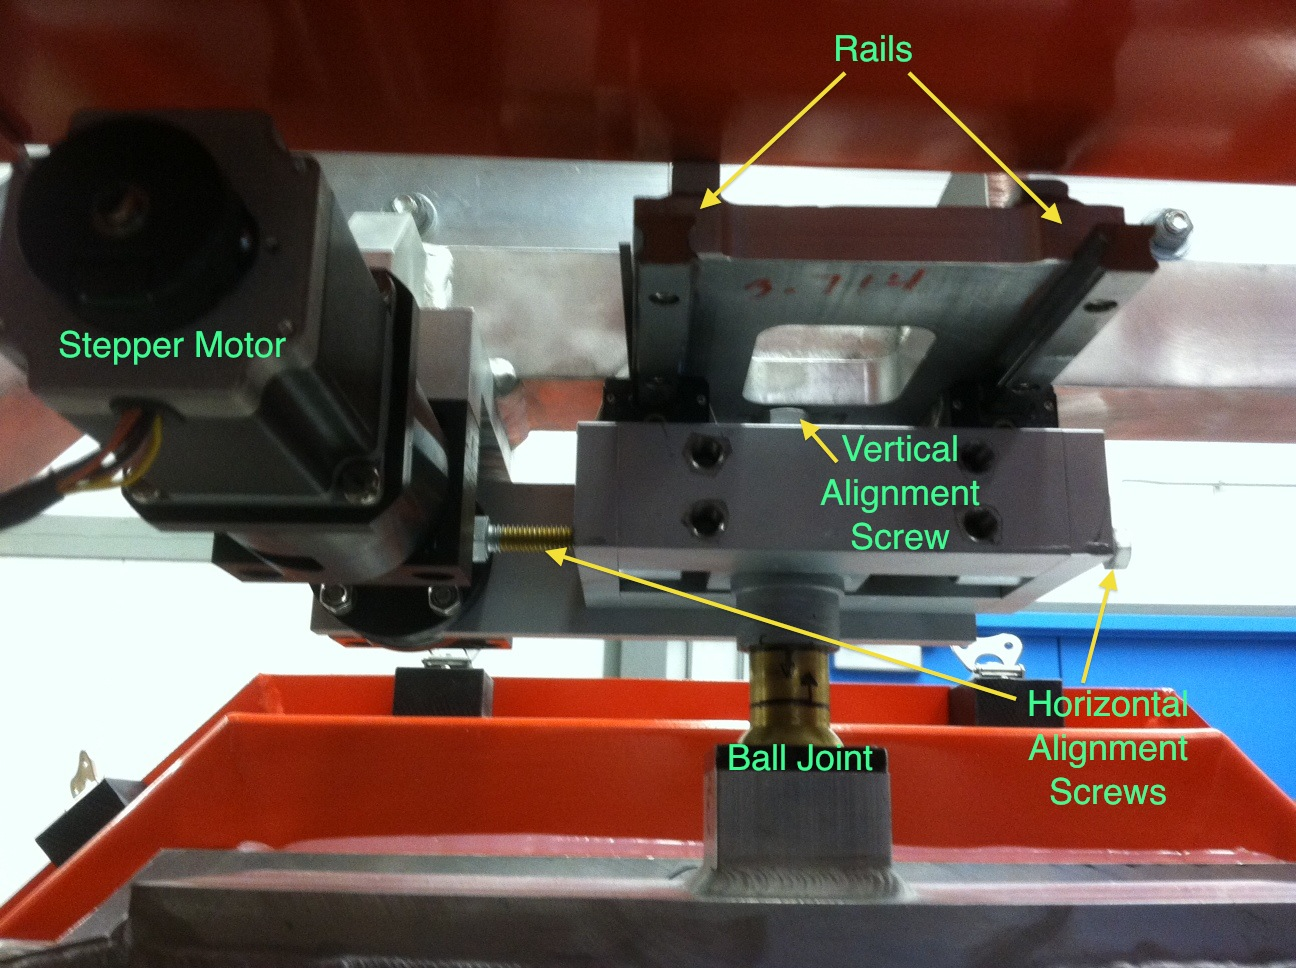
\includegraphics[width = 2.6in]{motorAss2Edit.JPG}
\caption{Motor assembly with relevant labels (the top motor assembly is shown).}  
\label{FigMotor}
\end{center}
\end{figure}



\section{Important Warnings/Notes}

First, some important warnings to keep in mind:
\begin{enumerate}
	\item Once the motion control set screws have been locked (this is done after the camera is aligned) {\bf DO NOT MOVE} the camera in any way except all forward or all backward (called vertical or along axis in the UI).
	Moving in any other way will likely break or bend things!
	\item The stepper motors supply enough thrust that they can and will {\bf CRUSH FINGERS} if you aren't careful!  Don't stick fingers around parts that are moving.
	\item If you need to turn off motion very quickly in the case of an emergency (fingers in the way of motion, etc!), click the green button on the electronics box.
		 This will kill the power to the Arduino and the motors and everything will stop immediately.
	\item Every time that you begin moving the camera, start small.  Test each motor individually +/-50 steps.  
		If you don't see a motor move, test that the screw isn't jammed by using a 1/2 inch socket to move the motor driver screw for that motor.
		Use the socket on the front side of the screw (opposite the motor).
		As easy way to see the screw move is to look at the pin on the end of each stepper motor (draw a black line on it to tell).
\end{enumerate}


\section{Startup Procedure}

\begin{figure}[h]
\begin{center}
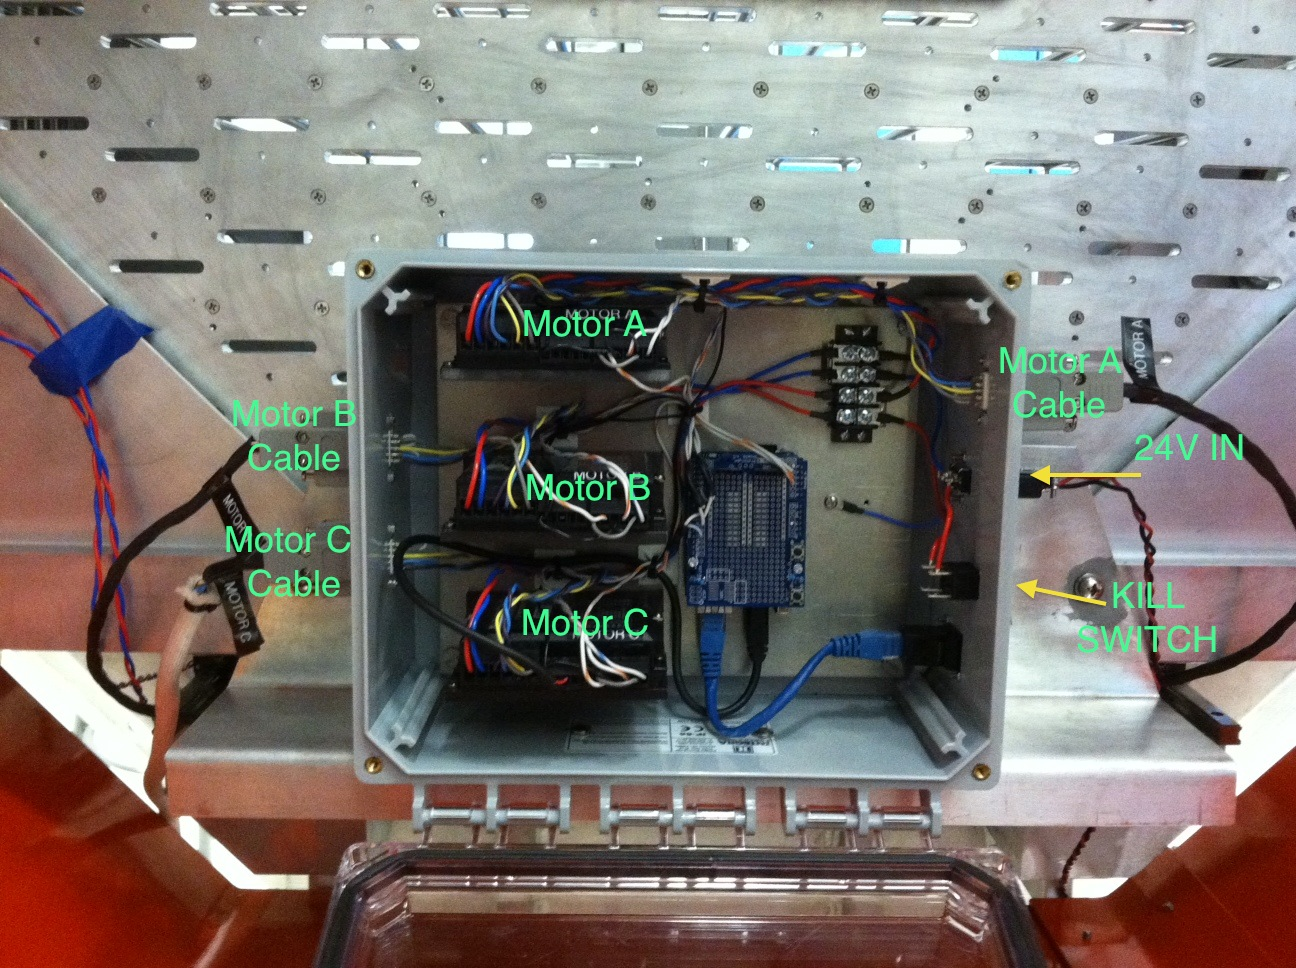
\includegraphics[width = 3.0in]{elecBox.JPG}
\caption{Electronics box located on the bottom of the back plane of the camera.}  
\label{FigElecBox}
\end{center}
\end{figure}


\begin{itemize}
	\item Power the electronics box.  You'll need to make sure that the green button on the side of the box is clicked-in.
		See Fig. \ref{FigElecBox} for a picture of the electronics box that houses the Arduino and stepper motor drivers (Fig. \ref{elecFit} shows the electrical schematic).  
	\item If everything powered up without problems, the LEDs on the motor drivers in the electronics box will be solid green. 
		If they aren't solid green see the troubleshooting section below.
	\item Navigate to the ip address that hosts the control html: [IP]/sd/MotionControl/
	\item Note that your first button click/command you make will not go through.  
		You will be asked instead to authenticate with the Arduino (default username, password is root, arduino).
	\item After authenticating you are good to go.  
		See the UI section below, you can now access the stored position, alignment, and range information for the camera or move it along its axis (i.e. all motors together).  
		If you need to move the camera in any orientation other than all-forward or all-back, click the 'ALIGNMENT MODE' button. 
	\item \underline{\it If you gave the wrong username/password when prompted you are not explicitly told.}
		You will be able to give the arduino commands but will not see any response messages or camera motion.
		Kill the browser and try again.
	\item To move only all-forward or all-back select the direction (+/-) and number of steps to move and have at it.  
		You will see a message that the movement completed successfully if there are no problems.
	\item For a more detailed discussion of the alignment procedure, see Sec. \ref{alignSec}.
\end{itemize}


\section{User Interface Commands}
	Position, range, and alignment information is stored in text files on an SD card mounted on the Arduino (specifically it is here  /mnt/sda1/*.txt).
	This information can then be accessed by the control software at any time or seen by directly ssh'ing into the Arduino.
	The position is the current position of the camera, this location is rewritten to the text file after every motion.
	The range is defined by users, it is meant as a fail-safe so that the motors can not drive motion past the hardware limits of the screw assembly.
	This only needs to be set once when a new Arduino or SD card is used.
	The alignment is also defined by users, it is the stored location where the camera was found to be properly 'aligned'.
	Again, only needs to be done once.
\begin{enumerate}
	\item[Get Range:] Load the camera range into the UI engine from the file on the Yun sd card.  Prints the stored range to the page in order of motor A, B, C. (range.txt)
	\item[Get Position:] Load the camera position into the UI engine from the file on the Yun sd card. Prints the current position to the page in order of motor A, B, C. (position.txt)
	\item[Get Alignment:] View the camera alignment position stored on the Yun sd card. Prints the stored alignment position to the page in order of motor A, B, C. (alignment.txt)
	\item[Set Alignment:] Write the current position as the alignment position to the Yun sd card. (alignment.txt)
	\item[Vertical:] Move all three motors by the same increment.
	\item[Pitch:] Move motor A in the requested direction. Move motor B in the opposite direction.
	\item[Roll:] Move both motors A and B in the same direction and C in the opposite direction.  There will be no movement along z of the camera, just a tilt.
	\item[A only:] Move only motor A.
	\item[B only:] Move only motor B.
	\item[C only:] Move only motor C.
	
	\item[Setting Range:] If for some reason the range hasn't been set correctly, do the folowing:
	\begin{enumerate} 
		\item[1.]SSH into the Yun (default username, password is root, arduino)
		\item[2.]Use vi to manually change the position.txt file (in /mnt/sda1/) to "20000L20000L20000".
		\item[3.]Use vi to manually change the range.txt file (in /mnt/sda1/) to "20000L20000L20000".
		\item[4.]Hit GETPOS on the webpage.
		\item[5.]Use the webpage to move the camera all the way back to the -Z limit.
		\item[6.]Change the position.txt file to "0L0L0".
		\item[7.]Hit GETPOS on the webpage.
		\item[8.]Use the webpage to move the camera all the way to the +Z limit.
		\item[9.]Hit GETPOS on the webpage.
		\item[10.]Manually change the range.txt file to the current position.
	\end{enumerate}
\end{enumerate}



\section{Alignment Procedure}
\label{alignSec}

Camera alignment can be broken up into rough and fine stages.
The rough alignment stage is performed by manually moving the camera up/down and left/right.
The fine alignment stages is then performed using the motion control web interface and the stepper motors.
After getting the camera near where you want it, you tighten down several screws.

\underline{Rough Alignment}:
\begin{enumerate}
	\item Push the camera to the height you want it.  
		This can be performed by ratcheting the two bottom vertical alignment screws beneath each ball pin (one direction moves the camera up, the other down).
		Note that the top alignment screw will need to be completely loose for this to work. 
		{\bf You have to keep the 2 lower screws perfectly in sync, or you will tilt the camera!}
		Use the 3/4 inch ratchet wrench with tape to do this (see Fig. \ref{figAlign}).
	\item Once the camera is at height, move the camera side-to-side to where you want it.
		You will need to loosen the horizontal alignment screws to do this - there are two on either side of the top ball pin and one around each lower ball pin.
		Movement will require your strong physicist muscles, no screw to help you here.
		Note that if it is already close to the center (should be) you can skip ahead to the fine alignment.
	\item {\bf Warning: }  There is a limitation on the horizontal motion in one direction due to the fan assembly.  
		When you are aligning the camera horizontally, make sure there is enough clearance between the fans and the metal octagon.
\end{enumerate}

\underline{Fine Alignment}
\begin{enumerate}
	\item Navigate to the MotionControl webpage from the [arduino ip]/sd webpage.
	\item Navigate to the alignment mode webpage (password is cta).
	\item Use the webpage to move the camera to a position where it is aligned.
	\item Lock down the vertical alignment screws beneath each ball pin.  
	\item {\bf Warning: } Make sure that the top vertical screw has clearance to move front-to-back.  
		See Fig. \ref{figAlign2}, don't be in the situation that the screw is in the hole and not down far enough to travel out of the hole.
	\item Lock in the horizontal alignment screws. 
		Use the 9/16 inch ratchet with tape for these guys.
	\item {\bf Warning 2: } Make sure that the top horizontal screw (left one) has clearance to move along the full z axis.  
		See Fig. \ref{FigMotor}, don't be in the case where this screw will hit the stepper motor assembly when moving along the z axis.
	\item If you need a longer screw to tighten in one of the horizontal directions, there is one in the telescope tool kit.
	\item {\bf After these screws are locked in the camera should only be run along the z axis (all-forward, all-back) - OR YOU WILL BEND/BREAK THE CAMERA!}
	\item Hit 'Set Alignment' to save the alignment position.  These alignment values will be loaded every time the system is started up, the only way to store new values is with this function (or manually changing the alignment.txt file).
\end{enumerate}


\begin{figure}[h]
\begin{center}
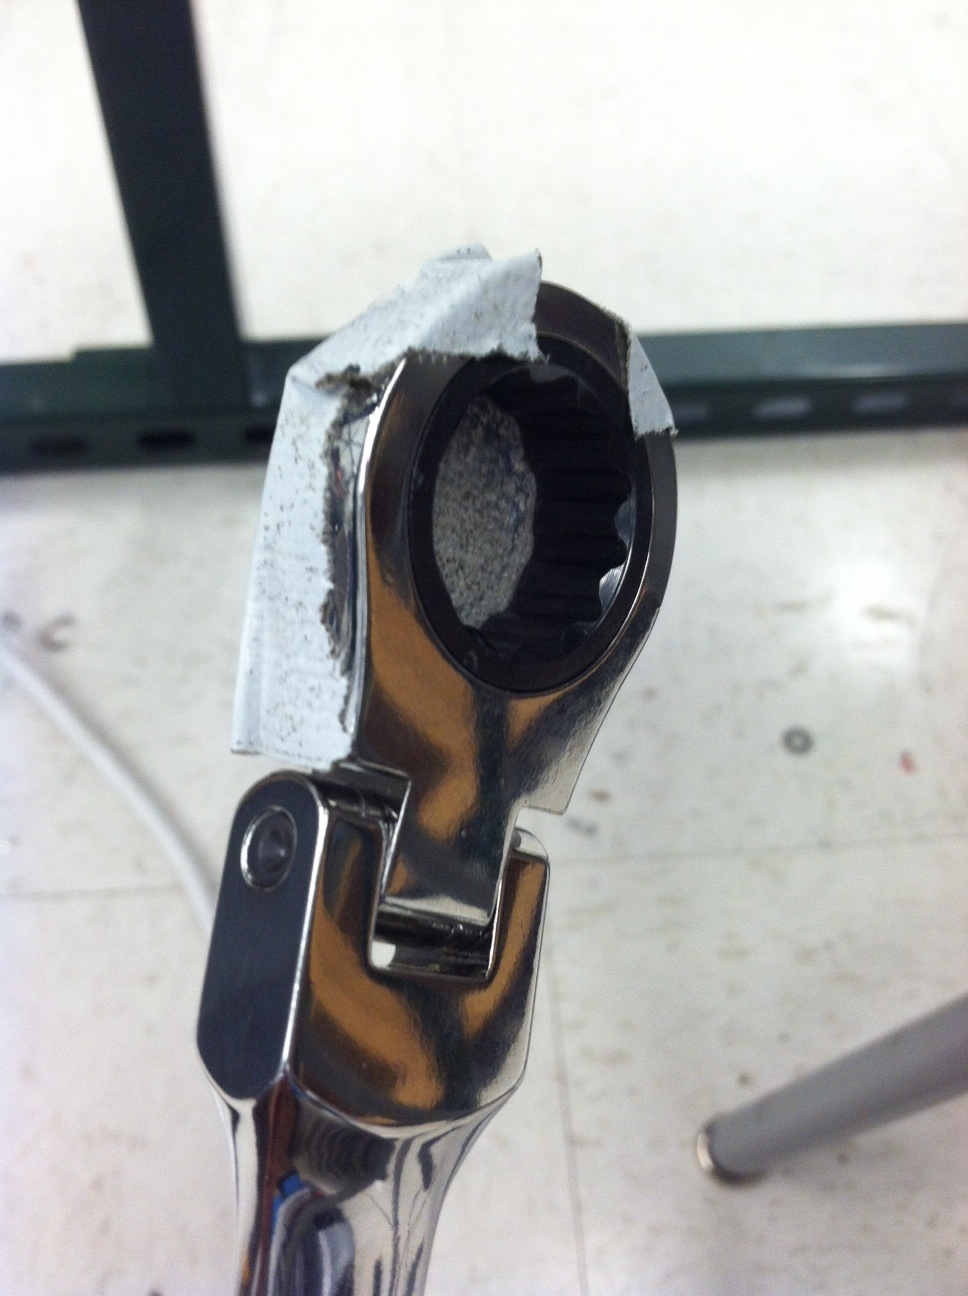
\includegraphics[width = 2.75in]{photoAlign1.JPG}
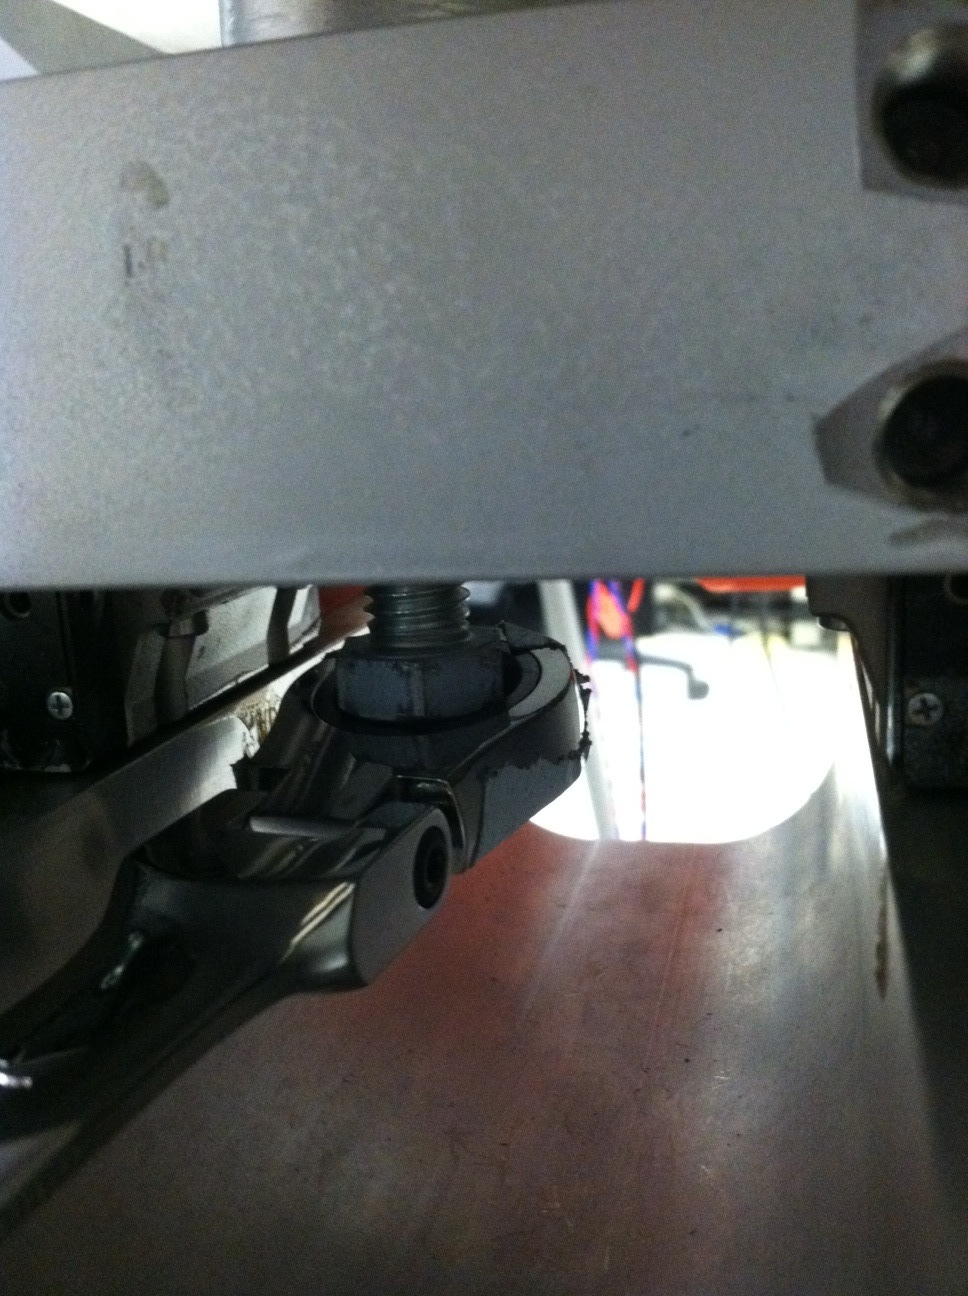
\includegraphics[width = 2.75in]{photoAlignTwo.JPG}
\caption{}  
\label{figAlign}
\end{center}
\end{figure}

\begin{figure}[h]
\begin{center}
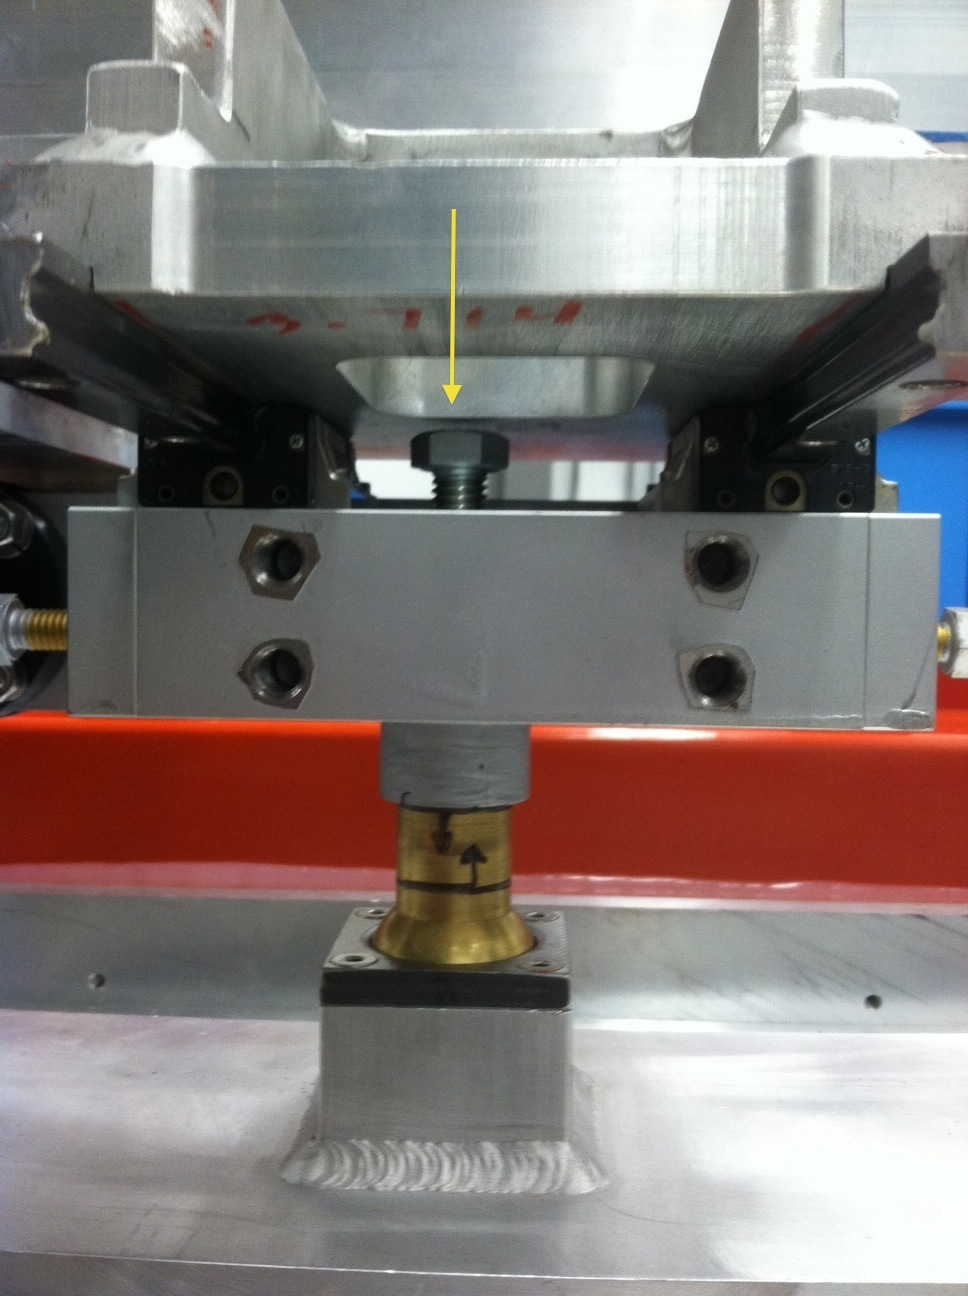
\includegraphics[width = 2.75in]{screwWarning.JPG}
\caption{}  
\label{figAlign2}
\end{center}
\end{figure}


\section{Troubleshooting}

\subsection{Problem with the motor drivers}

The LEDs on each of the three motor drivers in the electronics box will be solid green if everything is ok.
The fact that they are solid green means that they are powered, configured properly, and that they are sitting idle.  
If there is a problem in the configuration or hardware, it will likely show up here.

\begin{itemize}
	\item \underline{Blinking green}:  This means that the motor is powered and configured, but not sitting idle.  
		You may have to reload the Arduino sketch.
		The Arduino sketch is located here: https://github.com/wakely/sct-camera-software.  
		To upload the sketch you will have to download the Arduino IDE and be on a machine that can connect to the Arduino either via wifi or ethernet.
		If reloading the sketch doesn't work, reload the motor configuration (see Sec. \ref{SecConfig}).
 	\item \underline{Blinking red}:  Check to make sure that all three motor cables are properly connected.  
		A motor will be red if it can't find the hardware.  Otherwise, the motor driver may need to be reconfigured (see Sec. \ref{SecConfig}).
	\item \underline{Other combination of blinks and colors}:  See the LED codes listed in Fig. \ref{ledCodes} for insight.
	 	If reloading the motor driver configuration doesn't work you may have to change out the driver (see Sec. \ref{SecConfig}).  
		There is a spare in the telescope toolkit and you should be able to change it out, configure it, and be good to go.
\end{itemize}

\begin{figure}[h]
\begin{center}
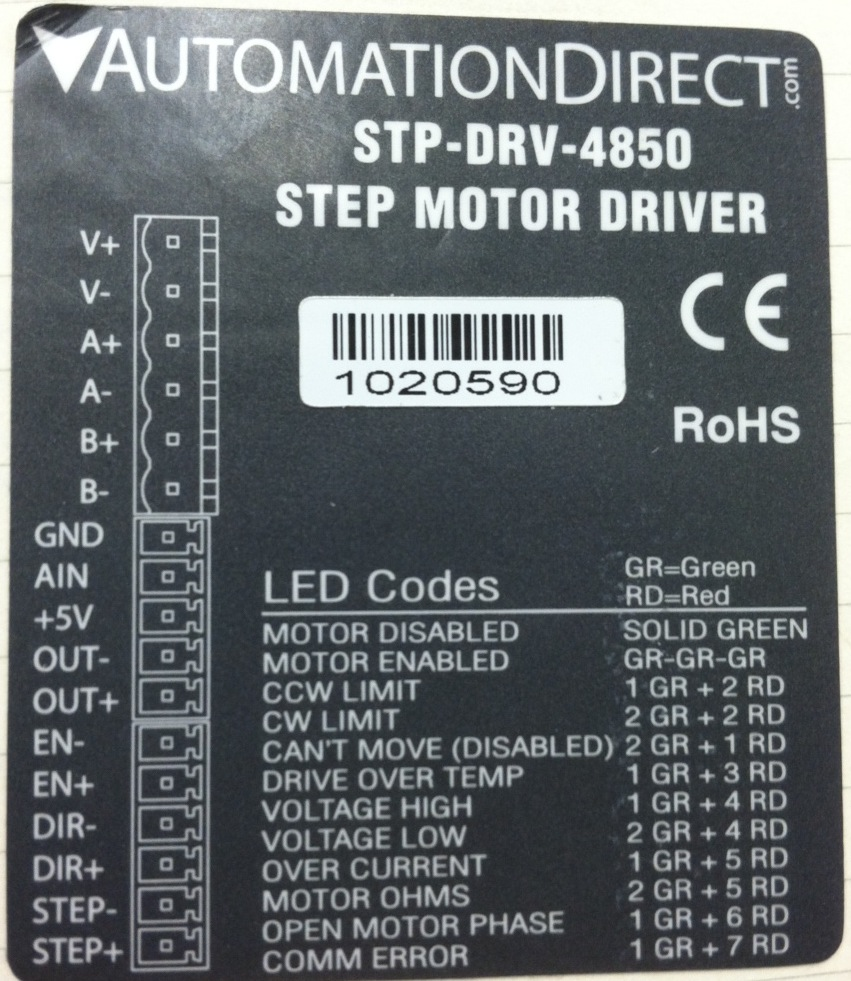
\includegraphics[width = 2.2in]{photoLedCodes.JPG}
\caption{Motor driver LED codes.}  
\label{ledCodes}
\end{center}
\end{figure}

\subsection{Problems with the stored camera information}

If power is lost at any time, it might be the case that one of the following files gets deleted: position.txt, range.txt, alignment.txt. 
The information in each of these files is loaded into memory when the program is started.
The Arduino sketch needs to know the camera location to move.
This is because there are limits set and calculated each time you request the telescope to move so you don't hit the limits.
Each of these files sits inside a directory on the Arduino SD care: /mnt/sda1\\[15pt]

If position.txt, or range.txt is missing:
\begin{enumerate}
\item[1.] Go into alignment mode if not there already and find the camera range (see "Setting Range" above).
\item[2.] Hit GETALGN to request the stored alignment position.
\item[3.] Manually move the camera to the alignment position.
\item[4.] Go back to the normal operation mode.
\end{enumerate}
If alignment.txt is missing realign the camera. Sorry :/. (This should never happen)

\subsection{Problems with a Yun}
See Sec. \ref{secYun} for more details.
If the $\mu$SD card is ok, you should be able to simply put the card into a new Yun and roll.


\subsection{Problem: motion sounds loud/grating}

Movement of the flange along the screw should not make loud noise or sound like grating.
If it sounds like metal-on-metal, stop moving the camera and investigate.
\begin{enumerate}
	\item Does the motion move smoothly when you twist the screw with a socket?  If you feel some tight spots along the 
		screw, the solution may be as simple as applying more lubrication.  Metal-on-metal isn't good.  
		There is some grease in the telescope toolkit in a can.  Use a popsicle stick (or something similar) to apply the
		grease near where the flange meets the screw and work in it by manually twisting the screw.
	\item If that doesn't solve the problem, make sure that the camera is not tilted.  
		The two ball pins on the bottom are what sets the camera level.  
		They need to be even, meaning they need to be the same number of turns from the bottom.  Check this!  
		If needed, work back from the bottom to the height you want.
	\item If neither of those fixes the problem, make sure that the screw has not been bent.  
		This would be a seriously pain to fix, so hopefully this isn't the case.  There is a spare screw in the toolkit.
		However, it will need to be cut to size.
\end{enumerate}


\section{Replacing a Yun with a new Yun that isn't configured}

\begin{figure}[h]
\begin{center}
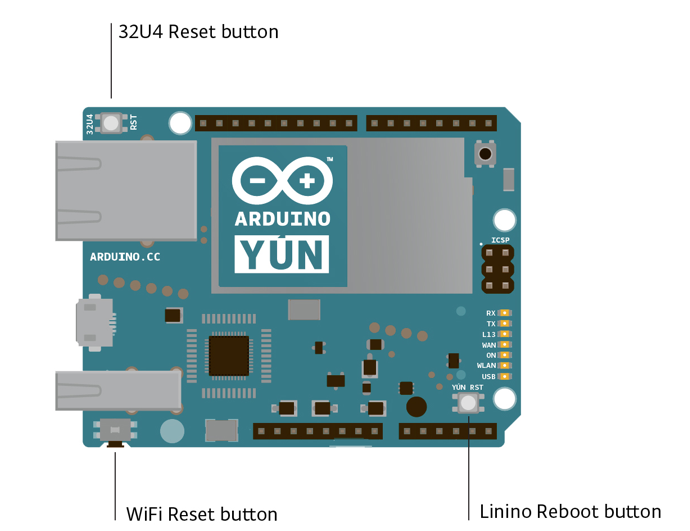
\includegraphics[width = 2.4in]{arduino1.png}
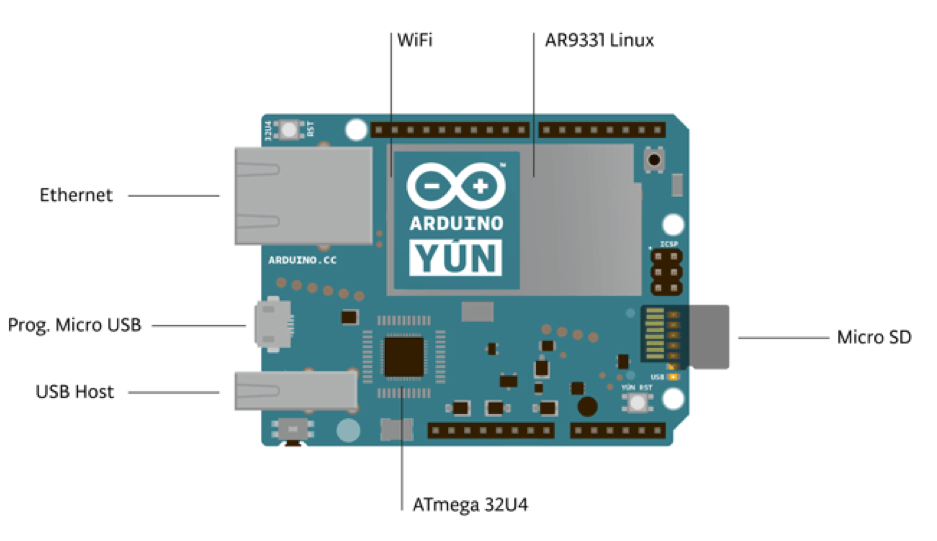
\includegraphics[width = 3.2in]{arduino2.png}
\caption{Arduino Yun button locations and overview schematic.}  
\label{YunFig}
\end{center}
\end{figure}

\label{secYun}
\begin{enumerate}
\item Replace the Arduino Yun in the electronics box (Fig. \ref{FigElecBox}) with a new one from the telescope toolkit.
	You will need to take the PCB shield on top of the Arduino off carefully, the wires soldered to this shield are tight and you don't want to bend the pins from the shield as you are taking it off.
	Once you have the shield off, the Arduino is mounted to the bottom aluminum plate in the box by three screws (flathead screwdriver needed for 4-40, 7/16'' screws).  
	Each of these screws additionally has a plastic standoff between the Arduino PCB and the plate, catch them as you are taking the Arduino off.
	Note that there are additional spacers and screws in the telescope toolkit if you lose one.
\item Plug the Yun into a laptop via micro usb to power it.
\item Look for the Yun's wifi network. If it doesn't appear, hold the wlan reset button until it blinks. 
	See Fig. \ref{YunFig} for reset button locations.
	Pressing all three buttons for several seconds will reset the Yun to factory defaults.
\item If the Yun's wifi network still doesn't appear try plugging the Yun ethernet into your LAN and connect to the Yun or Linino's network. Continue below as appropriate.\\
\item Are you using a Linino or Arduino?  Linino is an Arduino made by a competitor, it is essentially identical hardware with a slightly different operating system.
	An Arduino is made by arduino.cc whereas a Linino is made by arduino.org - you can see this on the body of the PSB.
        	\begin{itemize} 
		\item {\textbf{Linino:}} Open a browser and go to 192.168.240.1 and login to the Linino web UI. The default password is 'doghunter'.
		\item {\textbf{Arduino:}} Open a browser and go to arduino.local and login to the Arduino web UI. The default password is 'arduino' or 'arduino1'.
	\end{itemize}
\item \textbf{Continue Here:} Click on the advanced configuration at the top of the page.
\item Go to the network tab and click edit on the WAN panel.
\item Switch the network protocol to static ip.
\item Enter LAN ip reserved for the Yun along with the gateway ip and network mask. Hit save.
\item If required go to the wifi panel and disable the wifi.

\item If desired, set up the LAN to forward incoming requests from some port to the Yun ip.\\
\item \textbf{Loading the sketch:} If the previous Yun's sd card is still accessible just put it into the new Yun. Otherwise get a fresh sd card and download the Yun sd expander sketch (Google it).
\item If necessary find the Yun's ip address on the LAN and go that ip in your web browser. Then open up the Arduino IDE and select that same ip as the port. Upload the sd expander (and or the motion control sketch) if necessary.

\item After loading from the Arduino IDE you should see all the green lights on for the three motor drivers (not flashing).  
The motor drivers are located in the electronics box, see the wiring diagram below.

\item {\textbf{If you are using a Linino:}}  If the Ardiuno is a Linino you may have to create a symbolic link for the OS to know where to look for the website.  
After these steps you should be able to load the webpage via [Arduino IP] / [sd].  
If you can already connect, all is good already.
	\begin{itemize}
		\item ssh -Y root@[IP address]
		\item cd /www/
		\item ln -s /mnt/sda1/sd
	\end{itemize}
	
\item Note that with a fresh install you will need to physically create all the text files discussed above (position.txt, range.txt, alignment.txt).
	The procedure to do this is detailed in previous sections.
\end{enumerate}


\section{Configuring the Stepper Motor Drivers}
\label{SecConfig}

Reloading the configuration of a stepper motor driver will require a Windows machine and RJ11-to-Serial cable.
A cable is included in the telescope toolkit, a computer is not.
The various problem codes are shown in Fig \ref{ledCodes}, most of which will require you to (re-)configure the driver.
To do that, follow these steps:

\begin{enumerate}
\item Download SureStep Pro 1.0.8: \newline
http://support.automationdirect.com/products/surestep.html \newline
After you unzip the file the executable is there (note this needs to be on a Windows machine!)
The datasheet for the motor driver is also located here for the STP-DRV-4850: \newline
$www.automationdirect.com/static/manuals/surestepmanual/surestepdrive2\_datasheet.pdf$

\item Connect the computer to one of the properly configured driver motors, one that shows a green LED that isn't blinking. 
Use the RJ11-to-Serial cable for this and connect to one of the serial ports on the computer.

\item Click the 'Upload from Drive' to store the configuration from the working motor into the program.

\item Now connect the cable to the driver that isn't properly configured and click 'Download to Drive'.
This should reconfigure this driver with the proper settings from the prior driver.

\item If all the drivers are improperly configured you will have to manually set the configuration in the SureStep UI.  
Figure \ref{ConfigPic} shows the UI windows and configuration values for a working stepper motor.  
Input all these values into the various fields, connect to that driver, and then click 'Download to Drive'.
Note that we use a 'custom motor' configuration.
\end{enumerate}


\section{Removing the Inner Camera Structure}
We show here a step-by-step of removing the inner camera structure.  
Note that a lifting crane is absolutely necessary, the inner structure is very heavy.
We used a purple strap connected to an overhead crane that you will see in the pictures.

\begin{enumerate}
\item Ratchet down bottom screws (screws pushing up on the holding pins)
\item Move camera all the way forward
\item Allen wrench off the top piece holding in the pin.  See Figure \ref{figRemove1}.
\item Jiggle to get the ball to disconnect
\item Pop top ball joint out.  Now the top tilts forward.  See Figure \ref{figRemove2}.
\item Pull it up straight.
\item Pop out one of the two bottom pins (take it out 'leg-by-leg'). 
\item Lift manually out the other side pin
\item Don't drop it.  Seriously.
\end{enumerate}

\begin{figure}[h]
\begin{center}
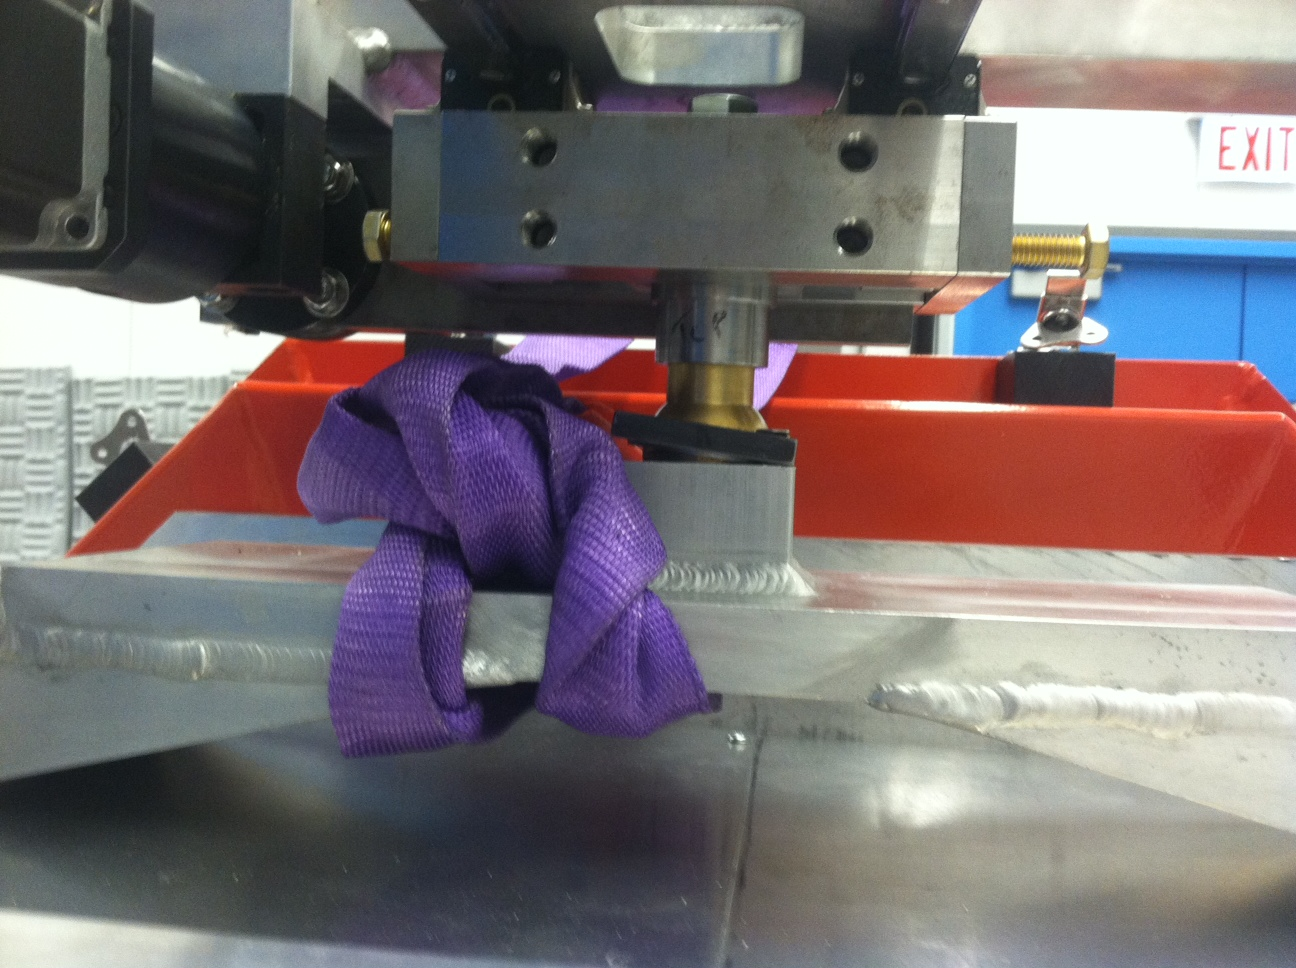
\includegraphics[width = 3in]{photo_2.png}
\end{center}
\caption{}  
\label{figRemove1}
\end{figure}


\begin{figure}[h]
\begin{center}
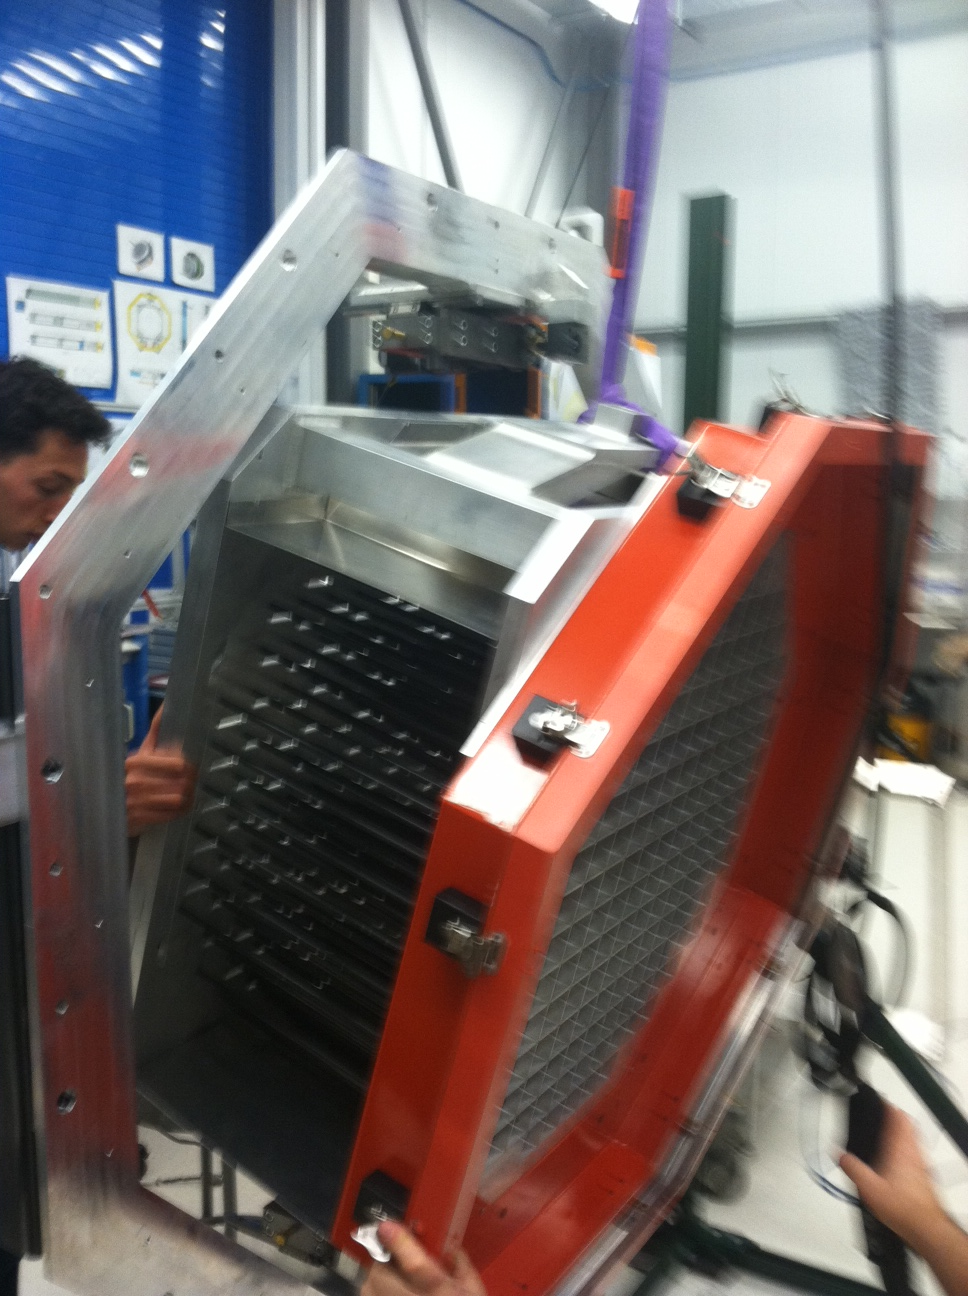
\includegraphics[width = 3in]{photo_3.png}
\end{center}
\caption{}  
\label{figRemove2}
\end{figure}


\section{Mounting the Inner Camera Structure}
We show here a step-by-step to mount the inner camera structure.  
Note that a lifting crane is absolutely necessary, the inner structure is very heavy.
We used a purple strap connected to an overhead crane that you will see in the pictures.

\begin{enumerate}
\item Move bottom motors all the way forward, the top motor all the way back.
\item Make sure the screws for the holding ball pins are ratcheted all the way down.
\item Put one lower ball joint in place
\item Bring the whole inner structure down to sink that one in
\item Pivot to put the other lower pin in
\item Now lower the inner structure all the way down until it is resting (you need clearance for the top pin)
\item Put the top ball pin in all the way and hold it there (you may have to ratched the screw up all the way)
\item Pivot the camera structure to put the ball into place 
\item Attach the ball pin holding frame with 1/8 inch allen
\item Ratchet up the bottom two nuts
\end{enumerate}


\newpage
\section{Fan Assembly Details}

The camera cooling system consists of two banks of 4 fans blowing through a water cooled radiator.
Each fan is an ebm-pabst model DV 6224 and the power is supplied by an Acopian power supply.
Each fan bank runs at a nominal voltage of 24V and draws 7A (14A for both banks, all 8 fans).
Figure \ref{fanPic} shows the terminal to connect the fan bank wires properly.

\begin{figure}[!th]
\begin{center}
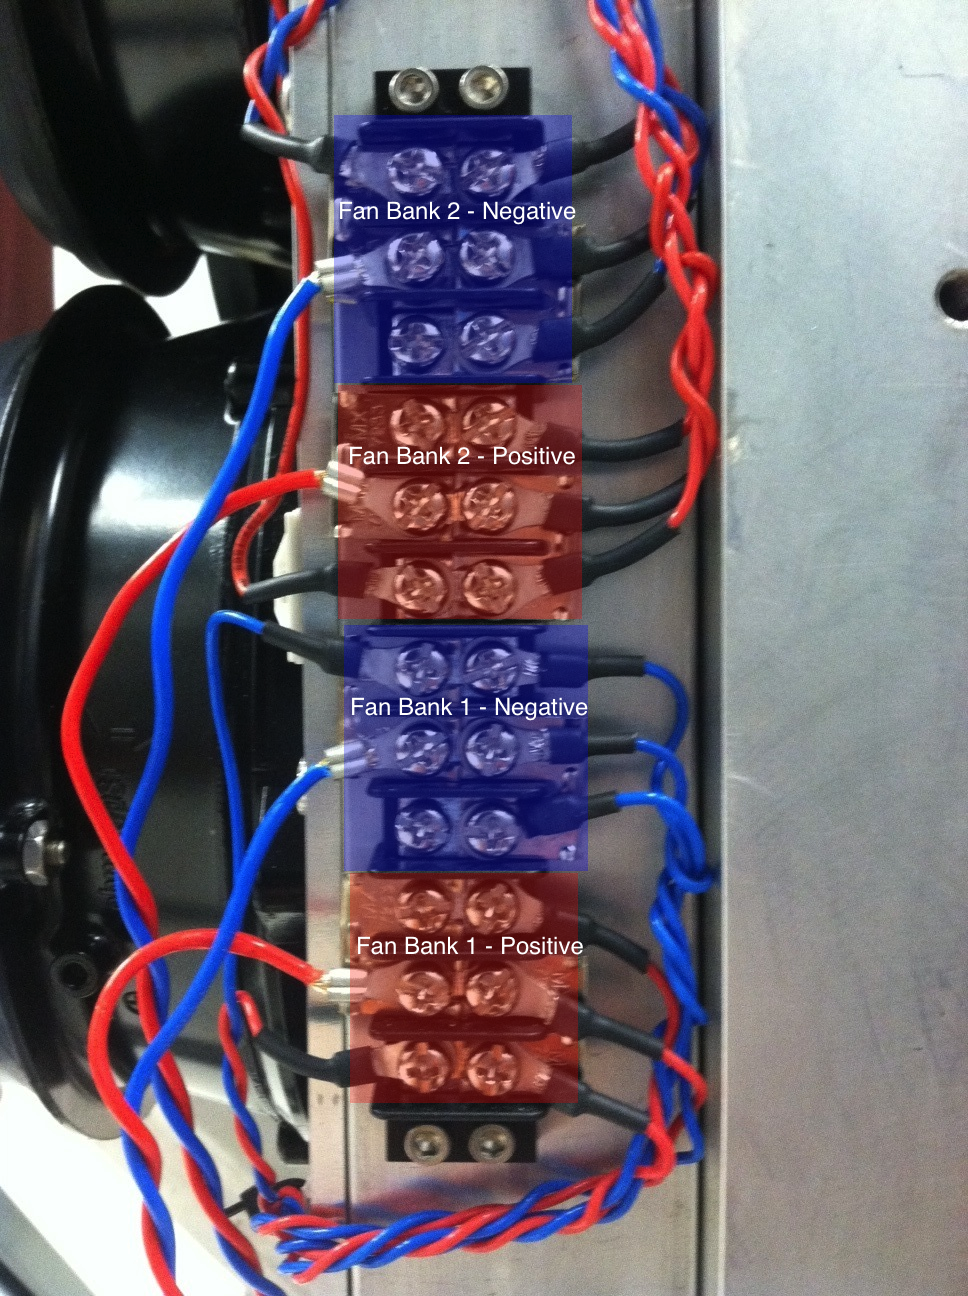
\includegraphics[width = 4in]{fanWiring.jpg}
\caption{Terminal block for fan assembly wiring.}  
\label{fanPic}
\end{center}
\end{figure}

\newpage
\section{Air Mitigation System - Baffles}

Since the camera isn't fully populated, we have manufactured baffles to force the air through the active area. 
Figure \ref{bafflePic2} shows the two types of baffles made.
Figure \ref{bafflePic} shows the optimal baffle orientation.
There is a front baffle that fits over the front of the camera areas that isn't populated and inner lattice baffles that fit into some of the empty module slots.

\begin{itemize}
	\item \underline{Front Baffle}: Secure the front baffle to the camera lattice using the eight holes around the perimeter.
		The baffle only fits onto the camera in one orientation and the intended orientation is marked clearly with the word 'TOP' on the back.
		Note that the lock nuts on the back of the baffle should not be removed under any circumstances.
		It is very difficult to put together once it is apart.

	\item \underline{Inner lattice camera baffles}:  The inner camera baffles are made with two holes in the back end.  
		This was done so that they could be inserted in the lattice module slots in either diagonal orientation.  
		The preferred orientation is shown in Fig. \ref{bafflePic}.  To install them:
		\begin{enumerate} 
			\item Slide the baffle into the lattice module slot until the front is flush with the focal plane.
			\item In the back of the camera you will need to secure the baffle with one of the red tipped thumb screws. 
				The baffle will have sagged a little so you will need to lift it in order to secure properly.
			\item Grab your trusty flathead and prop it up until one of the holes is centered in the slot.
				Use the thumb screw to secure.
		\end{enumerate}
\end{itemize}


\begin{figure}[h]
\begin{center}
\includegraphics[width = 2.5in]{frontBaffle.png}
\includegraphics[width = 2.5in]{innerBaffle.png}
\caption{Front baffle shown on the left. Inner camera baffle shown on the right being inserted into one of the module slots from the front of the camera. }  
\label{bafflePic2}
\end{center}
\end{figure}


\begin{figure}[h]
\begin{center}
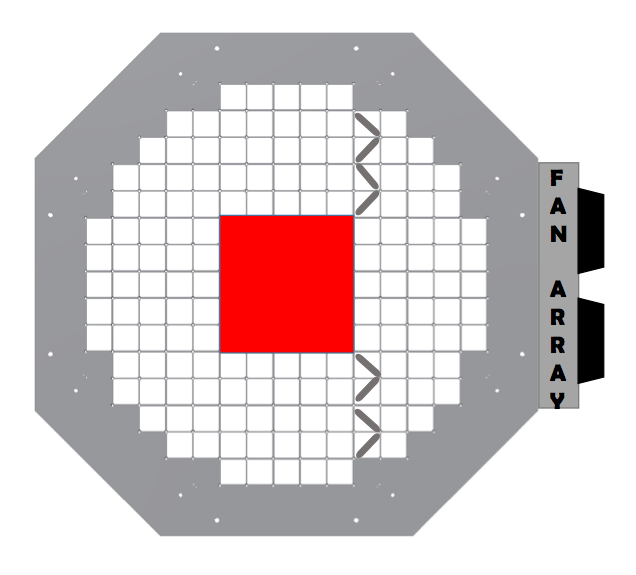
\includegraphics[width = 2.5in]{baffles.png}
\caption{Air baffle orientation.}  
\label{bafflePic}
\end{center}
\end{figure}



\newpage
\section{Tools in the Telescope Kit}

All the tools needed to drive each screw or bolt on the camera should be included in the camera toolbox. 
Additionally, there are spares for all the major components and connectors.
Have a look there first if you need something.
Here is what should be in there:

\begin{itemize}
	\item 3/4 inch flexible ratchet wrench with tape -- ball joint vertical centering screws for alignment
	\item 9/16 inch flexible ratchet wrench with tape -- ball joint horizontal centering screws for alignment
	\item 5/16 inch allen -- bolts for ball joint mount
	\item 7/32 inch allen -- Screw assembly bolts
	\item 2.5 mm allen -- slides
	\item 7/16 inch wrench (2x) -- screw flange bolts to connect screw to frame
	\item 3/16 inch wrench (2x) -- small wrenches for electronics box nuts
	\item 1/16 inch allen -- set screws for motor pins
	\item Phillips or flathead screwdriver -- everything else
	\item Spare $\mu$SD card
	\item Spare stepper motor driver + wiring terminals
	\item Spare stepper motor
	\item Touch-up paint and grease
	\item Spare electronics box pars (switch, ethernet mount, etc.)
	\item Spare horizontal alignment screw - allen head, extra long
	\item RJ11 to serial cable for stepper motor configuration
\end{itemize}

\newpage
\section{Electronics Box Wiring Diagram}
\begin{figure}[h]
\begin{center}
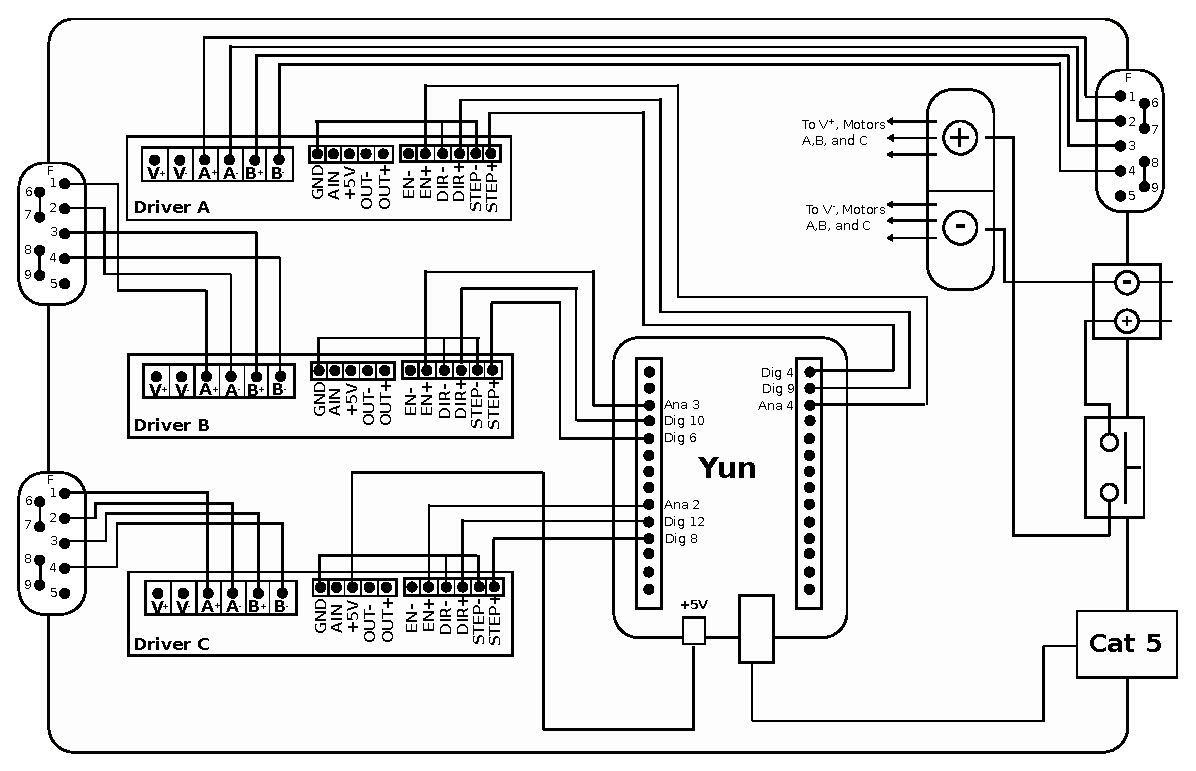
\includegraphics[width = 5.5in]{wiringDrawingUpdate.eps}
\caption{Wiring diagram for the electrical control box.}  
\label{elecFit}
\end{center}
\end{figure}


\begin{figure}[h]
\begin{center}
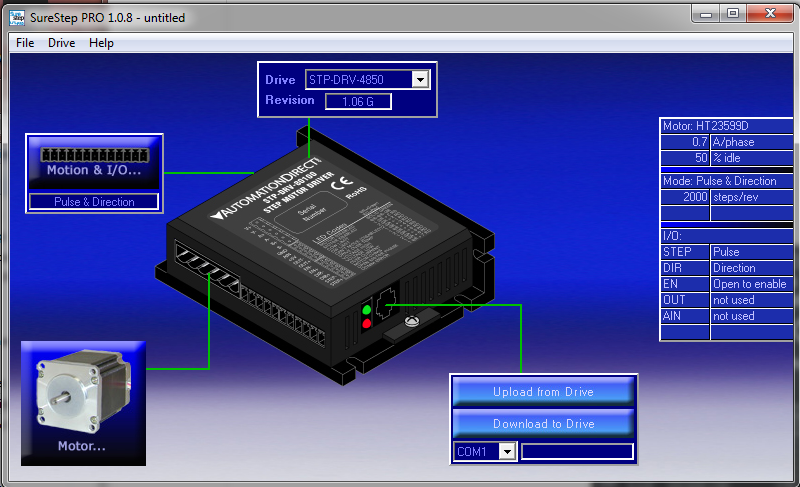
\includegraphics[width = 5in]{MotorConfiguration.png}
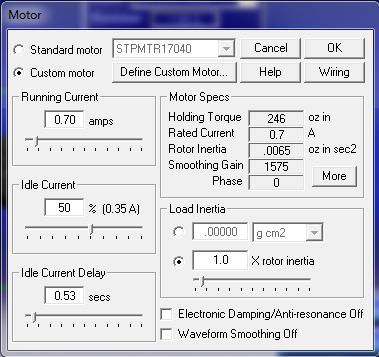
\includegraphics[width = 2.5in]{MotorConfig2.png}
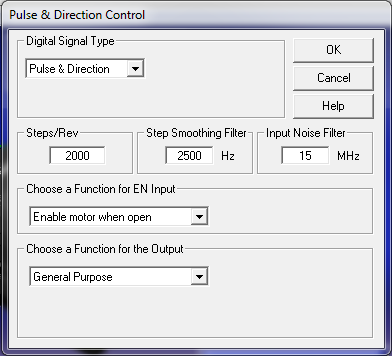
\includegraphics[width = 2.5in]{MotorConfig3.png}
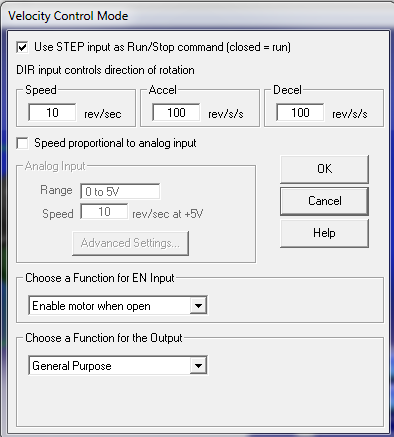
\includegraphics[width = 2.5in]{MotorConfig4.png}
\caption{SureStep 1.0.8 UI with the proper configuration settings.  The top photo shows the main UI and the other UIs are accessed via the 'Motion and I/O' button and 'Motor...' button.}  
\label{ConfigPic}
\end{center}
\end{figure}


\end{document}
